%beamer

% TODO:
% - VL-Folien einarbeiten
% - Weniger f_* etc. Theorie, mehr Aufgaben zwischendrin und zu Akzeptoren
% - Bessere Hinleitung zu Akzeptoren

% Comment/uncomment this line to toggle handout mode
\newcommand{\handout}{}

%% Beamer-Klasse im korrekten Modus
\ifdefined \handout
\documentclass[handout]{beamer} % Handout mode
\else
\documentclass{beamer}
\fi

%% UTF-8-Encoding
\usepackage[utf8]{inputenc}

\input{../framework/gbi-macros}
\usepackage[blue]{../framework/thwregex}
\usepackage{environ}
\usepackage{bm}
\usepackage{calc}
\usepackage{varwidth}
\usepackage{wasysym}
\usepackage{mathtools}


% Das ist der KIT-Stil
%\usepackage{../TutTexbib/beamerthemekit}
\usepackage[deutsch,titlepage0]{../framework/KIT/beamerthemeKITmod}
\TitleImage[width=\titleimagewd]{../figures/titlepage.jpg}
%\usetheme[deutsch,titlepage0]{KIT}

% Include PDFs
\usepackage{pdfpages}

% Libertine font (Original GBI font)
\usepackage{libertine}
%\renewcommand*\familydefault{\sfdefault}  %% Only if the base font of the document is to be sans serif

% Nicer math symbols
\usepackage{eulervm}
%\usepackage{mathpazo}
\renewcommand\ttdefault{cmtt} % Computer Modern typewriter font, see lecture slides.

\usepackage{csquotes}

%%%%%%

%% Schönere Schriften
\usepackage[TS1,T1]{fontenc}

%% Bibliothek für Graphiken
\usepackage{graphicx}

%% der wird sowieso in jeder Datei gesetzt
\graphicspath{{../figures/}}

%% Anzeigetiefe für Inhaltsverzeichnis: 1 Stufe
\setcounter{tocdepth}{1}

%% Hyperlinks
\usepackage{hyperref}
% I don't know why, but this works and only includes sections and NOT subsections in the pdf-bookmarks.
\hypersetup{bookmarksdepth=subsection} 

%\usepackage{lmodern}
\usepackage{colortbl}
\usepackage[absolute,overlay]{textpos}
\usepackage{listings}
\usepackage{forloop}
%\usepackage{algorithmic} % PseudoCode package 

\usepackage{tikz}
\usetikzlibrary{matrix}
\usetikzlibrary{arrows.meta}
\usetikzlibrary{automata}
\usetikzlibrary{tikzmark}
\usetikzlibrary{positioning}

% Why has no-one come up with this yet? I mean, seriously. -.-
\tikzstyle{loop below right} = [loop, out=-60,in=-30, looseness=7]
\tikzstyle{loop below left} = [loop, out=-150,in=-120, looseness=7]
\tikzstyle{loop above right} = [loop, out=60,in=30, looseness=7]
\tikzstyle{loop above left} = [loop, out=150,in=120, looseness=7]
\tikzstyle{loop right below} = [loop below right]
\tikzstyle{loop left below} = [loop below left]
\tikzstyle{loop right above} = [loop above right]
\tikzstyle{loop left above} = [loop above left]

% Needed for gbi-macros
\usepackage{xspace}

%%%%%%

%% Verbatim
\usepackage{moreverb}

%%%%%%%%%%%%%%%%%%%%%%%%%%%%%%%%%%%% Copy end

%% Tabellen
\usepackage{array}
\usepackage{multicol}
\usepackage{hhline}

%% Bibliotheken für viele mathematische Symbole
\usepackage{amsmath, amsfonts, amssymb}

%% Deutsche Silbentrennung und Beschriftungen
\usepackage[ngerman]{babel}

\usepackage{kbordermatrix}

% kbordermatrix settings
\renewcommand{\kbldelim}{(} % Left delimiter
\renewcommand{\kbrdelim}{)} % Right delimiter

\input{../config.tex}



% define custom \handout command flag if handout mode is toggled  #DirtyAsHellButWell...
\only<beamer:0>{\def\handout{}} %beamer:0 == handout mode

\newcommand{\R}{\mathbb{R}}
\newcommand{\N}{\mathbb{N}}
\newcommand{\Z}{\mathbb{Z}}
\newcommand{\Q}{\mathbb{Q}}
\newcommand{\BB}{\mathbb{B}}
\newcommand{\C}{\mathbb{C}}
\newcommand{\K}{\mathbb{K}}
\newcommand{\G}{\mathbb{G}}
\newcommand{\nullel}{\mathcal{O}}
\newcommand{\einsel}{\mathds{1}}
\newcommand{\Pot}{\mathcal{P}}
\renewcommand{\O}{\text{O}}

\def\word#1{\hbox{\textcolor{blue}{\texttt{#1}}}}
\let\literal\word
\def\mword#1{\hbox{\textcolor{blue}{$\mathtt{#1}$}}}  % math word
\def\sp{\scalebox{1}[.5]{\textvisiblespace}}
\def\wordsp{\word{\sp}}

%\newcommand{\literal}[1]{\textcolor{blue}{\texttt{#1}}}
\newcommand{\realTilde}{\textasciitilde \ }
\newcommand{\setsize}[1]{\ensuremath{\left\lvert #1 \right\rvert}}
\newcommand{\size}[1]{\setsize{#1}}  % Shame on you, TeXStudio...
\newcommand{\set}[1]{\left\{#1\right\}}
\newcommand{\tuple}[1]{\left(#1\right)}
\newcommand{\normalvar}[1]{\text{$#1$}}

% Modified by DJ
\let\oldemptyset\emptyset
\let\emptyset\varnothing % proper emptyset

\newcommand{\boder}{\ensuremath{\mathbin{\textcolor{blue}{\vee}}}\xspace}
\newcommand{\bund}{\ensuremath{\mathbin{\textcolor{blue}{\wedge}}}\xspace}
\newcommand{\bimp}{\ensuremath{\mathrel{\textcolor{blue}{\to}}}\xspace}
\newcommand{\bgdw}{\ensuremath{\mathrel{\textcolor{blue}{\leftrightarrow}}}\xspace}
\newcommand{\bnot}{\ensuremath{\textcolor{blue}{\neg}}\xspace}
\newcommand{\bone}{\ensuremath{\textcolor{blue}{1}}\text{}}
\newcommand{\bzero}{\ensuremath{\textcolor{blue}{0}}\text{}}
\newcommand{\bleftBr}{\ensuremath{\textcolor{blue}{\texttt{(}}}\text{}}
\newcommand{\brightBr}{\ensuremath{\textcolor{blue}{\texttt{)}}}\text{}}

% Fix of \b... commands:

\renewcommand{\boder}{\alor}
\renewcommand{\bund}{\aland}
\renewcommand{\bimp}{\alimpl}
\renewcommand{\bgdw}{\aleqv}
\renewcommand{\bnot}{\alnot}
\renewcommand{\bleftBr}{\alka}
\renewcommand{\brightBr}{\alkz}
\newcommand{\alA}{\word A}
\newcommand{\alB}{\word B}
\newcommand{\alC}{\word C}

\newcommand{\plB}{\plfoo{B}}
\newcommand{\plE}{\plfoo{E}}

\newcommand{\summe}[2]{\sum\limits_{#1}^{#2}}
\newcommand{\limes}[1]{\lim\limits_{#1}}

%\newcommand{\numpp}{\advance \value{weeknum} by -2 \theweeknum \advance \value{weeknum} by 2}
%\newcommand{\nump}{\advance \value{weeknum} by -1 \theweeknum \advance \value{weeknum} by 1}

\newcommand{\mycomment}[1]{}
\newcommand{\Comment}[1]{}

%% DISCLAIMER START 
% It is INSANELY IMPORTANT NOT TO DO THIS OUTSIDE BEAMER CLASS! IN ARTCILE DOCUMENTS, THIS IS VERY LIKELY TO BUG AROUND!
\makeatletter%
\@ifclassloaded{beamer}%
{
	% TODO 
	% no time... later.   (= never -.-)
	% redefine section to ignore multiple \section calls with the same title
}%
{
	\errmessage{ERROR: section command redefinition outside of beamer class document! Please contact the author of this code or read the F-ing disclaimer.}
}%
\makeatother%
%% DISCLAIMER END

\newcounter{abc}
\newenvironment{alist}{
  \begin{list}{(\alph{abc})}{
      \usecounter{abc}\setlength{\leftmargin}{8mm}\setlength{\labelsep}{2mm}
    }
}{\end{list}}


\newcommand{\stdarraystretch}{1.20}
\renewcommand{\arraystretch}{\stdarraystretch}  % for proper row spacing in tables

\newcommand{\morescalingdelimiters}{   % for proper \left( \right) typography
	\delimitershortfall=-1pt  
	\delimiterfactor=1
}

\newcommand{\centered}[1]{\vspace{-\baselineskip}\begin{center}#1\end{center}\vspace{-\baselineskip}}

% for \implitem and \item[bla] stuff to look right:
\setbeamercolor*{itemize item}{fg=black}
\setbeamercolor*{itemize subitem}{fg=black}
\setbeamercolor*{itemize subsubitem}{fg=black}

\setbeamercolor*{description item}{fg=black}
\setbeamercolor*{description subitem}{fg=black}
\setbeamercolor*{description subsubitem}{fg=black}

\renewcommand{\qedsymbol}{\textcolor{black}{\openbox}}

\renewcommand{\mod}{\mathop{\textbf{mod}}}
\renewcommand{\div}{\mathop{\textbf{div}}}

\newcommand{\ceil}[1]{\left\lceil#1\right\rceil}
\newcommand{\floor}[1]{\left\lfloor#1\right\rfloor}
\newcommand{\abs}[1]{\left\lvert #1 \right\rvert}
\newcommand{\Matrix}[1]{\begin{pmatrix} #1 \end{pmatrix}}
\newcommand{\braced}[1]{\left\lbrace #1 \right\rbrace}

% "something" placeholder. Useful for repairing spacing of operator sections, like `\sth = 42`.
\def\sth{\vphantom{.}}

\def\fract#1/#2 {\frac{#1}{#2}} % ! Trailing space is crucial!
\def\dfract#1/#2 {\dfrac{#1}{#2}} % ! Trailing space is crucial!

\newcommand{\Mid}{\;\middle|\;}

\let\after\circ



\def\·{\cdot}
\def\*{\cdot}
\def\?>{\ensuremath{\rightsquigarrow}}  % Fuck you, Latex
\def\~~>{\ensuremath{\rightsquigarrow}}  

\newcommand{\tight}[1]{{\renewcommand{\arraystretch}{0.76} #1}}
\newcommand{\stackedtight}[1]{\renewcommand{\arraystretch}{0.76} \begin{matrix} #1 \end{matrix} }
\newcommand{\stacked}[1]{\begin{matrix} #1 \end{matrix} }
\newcommand{\casesl}[1]{\delimitershortfall=0pt  \left\lbrace\hspace{-.3\baselineskip}\begin{array}{ll} #1 \end{array}\right.}
\newcommand{\casesr}[1]{\delimitershortfall=0pt  \left.\begin{array}{ll} #1 \end{array}\hspace{-.3\baselineskip}\right\rbrace}
\newcommand{\caseslr}[1]{\delimitershortfall=0pt  \left\lbrace\hspace{-.3\baselineskip}\begin{array}{ll} #1 \end{array}\hspace{-.3\baselineskip}\right\rbrace}

\def\q#1uad{\ifnum#1=0\relax\else\quad\q{\the\numexpr#1-1\relax}uad\fi}
% e.g. \q1uad = \quad, \q2uad = \qquad etc.

\newcommand{\qqquad}{\q3uad}
\newcommand{\minusquad}{\hspace{-1em}}

%% Placeholder utils
% \§{#1}   Saves #1 as placeholder and prints it
% \.       Prints an \hphantom with the size of the recalled placeholder.
\def\indentstring{}
\def\§#1{\def\indentstring{#1}#1}
\def\.{{$\hphantom{\text{\indentstring}}$}}
%% Placeholder utils end

\newcommand{\impl}{\ifmmode\ensuremath{\mskip\thinmuskip\Rightarrow\mskip\thinmuskip}\else$\Rightarrow$\fi\xspace}
\newcommand{\Impl}{\ifmmode\implies\else$\Longrightarrow$\fi\xspace}

\newcommand{\derives}{\Rightarrow}

\newcommand{\gdw}{\ifmmode\mskip\thickmuskip\Leftrightarrow\mskip\thickmuskip\else$\Leftrightarrow$\fi\xspace}
\newcommand{\Gdw}{\ifmmode\iff\else$\Longleftrightarrow$\fi\xspace}

% Legacy code from the algo tutorial slides. Perhaps useful. Try with care.
\mycomment{
	\newcommand{\impl}{\ifmmode\ensuremath{\mskip\thinmuskip\Rightarrow\mskip\thinmuskip}\else$\Rightarrow$\xspace\fi}  
	\newcommand{\Impl}{\ifmmode\implies\else$\Longrightarrow$\xspace\fi}
	
	\newcommand{\gdw}{\ifmmode\mskip\thickmuskip\Leftrightarrow\mskip\thickmuskip\else$\Leftrightarrow$\xspace\fi}
	\newcommand{\Gdw}{\ifmmode\iff\else$\Longleftrightarrow$\xspace\fi}
}
	
\newcommand{\gdwdef}{\ifmmode\mskip\thickmuskip:\Leftrightarrow\mskip\thickmuskip\else:$\Leftrightarrow$\xspace\fi}
\newcommand{\Gdwdef}{\ifmmode\mskip\thickmuskip:\Longleftrightarrow\mskip\thickmuskip\else:$\Longleftrightarrow$\xspace\fi}

\newcommand{\symbitemnegoffset}{\hspace{-.5\baselineskip}}
\newcommand{\implitem}{\item[\impl\symbitemnegoffset]}
\newcommand{\Implitem}{\item[\Impl\symbitemnegoffset]}


\newcommand{\forcenewline}{\mbox{}\\}

\newcommand{\bfalert}[1]{\textbf{\alert{#1}}}
\let\elem\in   % I'm a Haskell freak. Don't judge me. :P


\def\|#1|{\text{\normalfont #1}}  % | steht für senkrecht (anstatt kursiv wie sonst im math mode)


% proper math typography
\newcommand{\functionto}{\longrightarrow}
\renewcommand{\geq}{\geqslant}
\renewcommand{\leq}{\leqslant}
\let\oldsubset\subset
\renewcommand{\subset}{\subseteq} % for all idiots out there using subset

\newenvironment{threealign}{%
	\[
	\begin{array}{r@{\ }c@{\ }l}
}{%
	\end{array}	
	\]
}

\newcommand{\concludes}{ \\ \hline  }
\newcommand{\deduction}[1]{
	\begin{varwidth}{.8\linewidth}
		\begin{tabular}{>{$}c<{$}}
			#1
		\end{tabular}
	\end{varwidth}	
}

\definecolor{hoareorange}{rgb}{1,.85,.6}
\newcommand{\hoareassert}[1]{\setlength{\fboxsep}{1pt}\setlength{\fboxrule}{-1.4pt}\fcolorbox{white}{hoareorange}{\ensuremath{\{\;#1\;\}}}\setlength\fboxrule{\defaultfboxrule}\setlength{\fboxsep}{3pt}}

\newcommand{\mailto}[1]{\href{mailto:#1}{{\textcolor{blue}{\underline{#1}}}}}
\newcommand{\urlnamed}[2]{\href{#2}{\textcolor{blue}{\underline{#1}}}}
\renewcommand{\url}[1]{\urlnamed{#1}{#1}}

\newcommand{\hanging}{\hangindent=0.7cm}
\newcommand{\indented}{\hanging}


% \hstretchto prints #2 left-aligned into a box of the width of #1
\def\hstretchto#1#2{%
	\mbox{}\vphantom{#2}\rlap{#2}\hphantom{#1}%
}

\def\vstretchto#1#2{%
	\mbox{}\hphantom{#2}\smash{#2}\vphantom{#1}%
}

% \hstretchtocentered prints #2 centered into a box of the width of #1
\def\hstretchtocentered#1#2{%
	\mbox{}\vphantom{#2}\scalebox{0.5}{\hphantom{#1}}\clap{#2}\scalebox{0.5}{\hphantom{#1}}%
}

% vertical centering
\newcommand{\vertcenter}[1]{%
	\ensuremath{\vcenter{\hbox{#1}}}%
}


%requires \thisyear to be defined (s. config.tex)!
\edef\nextyear{\the\numexpr\thisyear+1\relax}


% --- \frameheight constant ---
\newlength\fullframeheight
\newlength\framewithtitleheight
\setlength\fullframeheight{.92\textheight}
\setlength\framewithtitleheight{.86\textheight}

\newlength\frameheight
\setlength\frameheight{\fullframeheight}

\let\frametitleentry\relax
\let\oldframetitle\frametitle
\def\newframetitle#1{\global\def\frametitleentry{#1}\if\relax\frametitleentry\relax\else\setlength\frameheight{\framewithtitleheight}\fi\oldframetitle{#1}}
\let\frametitle\newframetitle

\def\newframetitleoff{\let\frametitle\oldframetitle}
\def\newframetitleon{\let\frametitle\newframetitle}
% --- \frameheight constant end ---

\newcommand{\fakeframetitle}[1]{%
	\vspace{-2.05\baselineskip}%
	{\Large \textbf{#1}} \\%
	\smallskip
}



\newenvironment{headframe}{\Huge THIS IS AN ERROR. PLEASE CONTACT THE ADMIN OF THIS TEX CODE. (headframe env def failed)}{}
\RenewEnviron{headframe}[1][]{
	\begin{frame}\frametitle{\ }
		\centering
		\Huge\textbf{\textsc{\BODY} \\
		}
		\Large {#1}
		\frametitle{\ }
	\end{frame}
}


\makeatletter
% Provides color if undefined.
\newcommand{\colorprovide}[2]{%
	\@ifundefinedcolor{#1}{\colorlet{#1}{#2}}{}}
\makeatother


\colorprovide{lightred}{red!30}
\colorprovide{lightgreen}{green!40}
\colorprovide{lightyellow}{yellow!50}
\colorprovide{lightblue}{blue!10}
\colorprovide{beamerlightred}{lightred}
\colorprovide{beamerlightgreen}{lightgreen}
\colorprovide{beamerlightyellow}{lightyellow}
\colorprovide{beamerlightblue}{lightblue}
\colorprovide{fullred}{red!60}
\colorprovide{fullgreen}{green}
\definecolor{darkred}{RGB}{115,48,38}
\definecolor{darkgreen}{RGB}{48,115,38}
\definecolor{darkyellow}{RGB}{100,100,0}

\only<handout:0>{\colorlet{adaptinglightred}{beamerlightred}}
\only<handout:0>{\colorlet{adaptinglightgreen}{beamerlightgreen}}
\only<handout:0>{\colorlet{adaptinglightyellow}{beamerlightyellow}}
\only<handout:0>{\colorlet{adaptinglightblue}{beamerlightblue}}
\only<beamer:0>{\colorlet{adaptinglightred}{lightred}}
\only<beamer:0>{\colorlet{adaptinglightgreen}{lightgreen}}
\only<beamer:0>{\colorlet{adaptinglightyellow}{lightyellow}}
\only<beamer:0>{\colorlet{adaptinglightblue}{lightblue}}
\only<handout:0>{\colorlet{adaptingred}{lightred}}
\only<beamer:0>{\colorlet{adaptingred}{fullred}}
\only<handout:0>{\colorlet{adaptinggreen}{lightgreen}}
\only<beamer:0>{\colorlet{adaptinggreen}{fullgreen}}



\newcommand{\TrueQuestion}[1]{
	\TrueQuestionE{#1}{}
}

\newcommand{\YesQuestion}[1]{
	\YesQuestionE{#1}{}
}

\newcommand{\FalseQuestion}[1]{
	\FalseQuestionE{#1}{}
}

\newcommand{\NoQuestion}[1]{
	\NoQuestionE{#1}{}
}

\newcommand{\DependsQuestion}[1]{
	\DependsQuestionE{#1}{}
}

\newcommand{\QuestionVspace}{\vspace{4pt}}
\newcommand{\QuestionParbox}[1]{\begin{varwidth}{.85\linewidth}#1\end{varwidth}}
\newcommand{\ExplanationParbox}[1]{\begin{varwidth}{.97\linewidth}#1\end{varwidth}}
\colorlet{questionlightgray}{gray!23}
\let\defaultfboxrule\fboxrule

% #1: bg color
% #2: fg color short answer
% #3: short answer text
% #4: question
% #5: explanation
\newcommand{\GenericQuestion}[5]{
	\setlength\fboxrule{2pt}
	\only<+|handout:0>{\hspace{-2pt}\fcolorbox{white}{questionlightgray}{\QuestionParbox{#4} \quad\textbf{?}}}
	\visible<+->{\hspace{-2pt}\fcolorbox{white}{#1}{\QuestionParbox{#4} \quad\textbf{\textcolor{#2}{#3}}} \if\relax#5\relax\else\ExplanationParbox{#5}\fi} \\
	\setlength\fboxrule{\defaultfboxrule}
}

% #1: Q text
% #2: Explanation
\newcommand{\TrueQuestionE}[2]{
	\GenericQuestion{adaptinglightgreen}{darkgreen}{Wahr.}{#1}{#2}
}

% #1: Q text
% #2: Explanation
\newcommand{\YesQuestionE}[2]{
	\GenericQuestion{adaptinglightgreen}{darkgreen}{Ja.}{#1}{#2}
}

% #1: Q text
% #2: Explanation
\newcommand{\FalseQuestionE}[2]{
	\GenericQuestion{adaptinglightred}{darkred}{Falsch.}{#1}{#2}
}

% #1: Q text
% #2: Explanation
\newcommand{\NoQuestionE}[2]{
	\GenericQuestion{adaptinglightred}{darkred}{Nein.}{#1}{#2}
}

% #1: Q text
% #2: Explanation
\newcommand{\DependsQuestionE}[2]{
	\GenericQuestion{adaptinglightyellow}{darkyellow}{Je nachdem!}{#1}{#2}
}

% #1: Q text
% #2: Answer
\newcommand{\ContentQuestion}[2]{
	\GenericQuestion{adaptinglightblue}{black}{\minusquad}{#1}{#2}
}

\ifnum\thisyear=2021 \else \errmessage{Old ILIAS link inside preamble. Please update.} \fi

\newcommand{\ILIAS}{\urlnamed{ILIAS}{\myILIASurl}\xspace}
\newcommand{\Klausurtermin}{\myKlausurtermin\xspace}

\newcommand{\Socrative}{\ifdefined\mysocrativeroom \only<handout:0>{socrative.com $\quad \~~> \quad $ Student login \\ Raumname:  \mysocrativeroom\\ \medskip}\else\fi}

\newcommand{\thasse}[1]{
	\ifdefined\ThassesTut #1\xspace \else\fi
}
\newcommand{\daniel}[1]{
	\ifdefined\DanielsTut #1\xspace \else\fi
}
\newcommand{\thassedaniel}[2]{\ifdefined\ThassesTut #1\else\ifdefined\DanielsTut #2\fi\fi\xspace}

\ifdefined\ThassesTut \ifdefined\DanielsTut \errmessage{ERROR: Both ThassesTut and DanielsTut flags are set. This is most likely an error. Please check your config.tex file.} \else \fi \else \ifdefined\DanielsTut \else \errmessage{ERROR: Neither ThassesTut  nor DanielsTut flags are set. This is most likely an error. Please check your config.tex file.} \fi\fi

%\newcommand{\sgn}{\text{sgn}}

%%%%%%%%%%%% INHALT %%%%%%%%%%%%%%%%

%% Wochennummer
\newcounter{weeknum}

%% Titelinformationen
\title[GBI-Tutorium \mytutnumber, Woche \theweeknum]{Grundbegriffe der Informatik \\ Tutorium \mytutnumber}

\subtitle{Woche \theweeknum\xspace |\xspace\mydate{\theweeknum} \\ \myname \ \  \normalfont (\mailto{\mymail})}
\author[\myname]{\myname}
\institute{KIT -- Karlsruher Institut für Technologie}
\date{\mydate{\theweeknum}\ }

% Modified, DJ (better safe than sorry)
\AuthorTitleSep{ – }

%% Titel einfügen
\newcommand{\titleframe}{\frame{\titlepage}}

%% Alles starten mit \starttut{X}
\newcommand{\starttut}[1]{\setcounter{weeknum}{#1}\pdfinfo{
		/Author (\myname)
		/Title  (GBI-Tutorium \mytutnumber, Woche \theweeknum)
	}\titleframe\frame{\frametitle{Inhalt}\tableofcontents} \AtBeginSection[]{%
		\begin{frame}{Wo sind wir gerade?}
		\tableofcontents[currentsection]
	\end{frame}\addtocounter{framenumber}{-1}}}


\newcommand{\framePrevEpisode}{
\begin{headframe}
	\mylasttimestext
\end{headframe}
}

\newcommand{\lastframetitled}[6]{
	\frame{\frametitle{#6}
		\vspace{-#2\baselineskip}
		\begin{figure}[H]
			\centering
			\LARGE \textbf{\textsc{#5}} \\
			\vspace{.2\baselineskip}
			\includegraphics[#1]{#3}
			\vspace{-6pt}
			\begin{center}
				\small \url{#4} 
			\end{center}
		\end{figure} 
	}
}

% #1 number
% #2 title 
% #3 vspace (positive) without unit (\baselineskip)
\newcommand{\xkcdframe}[3]{
	\lastframetitled{width=.96\textwidth}{#3}{xkcd/#1}{http://xkcd.com/#1}{}{#2}
}

\newcommand{\xkcdframevert}[3]
{
	\lastframetitled{height=.96\frameheight}{#3}{xkcd/#1}{http://xkcd.com/#1}{}{#2}
}

% #1 number
% #2 title 
% #3 vspace (positive) without unit (\baselineskip)
% #4 \includegraphics[] optional parameters
\newcommand{\xkcdframecustom}[4]
{
	\lastframetitled{#4}{#3}{xkcd/#1}{http://xkcd.com/#1}{}{#2}
}

\newcommand{\slideThanks}{
	\begin{frame}
	\frametitle{Credits}
	\begin{block}{}
		An der Erstellung des Foliensatzes haben mitgewirkt:\\[1em]
		Daniel Jungkind \\
		Thassilo Helmold \\
		Philipp Basler \\
		Nils Braun \\
		Dominik Doerner \\
		Ou Yue \\
		Max Schweikart
	\end{block}
\end{frame}
}

%% Wörter DEPRECATED! DO NOT USE
\newcommand{\code}[1]{$\mathbf{#1}$}

\morescalingdelimiters

\begin{document}
\starttut{12}

\section{Rückblick}

\begin{frame}{Zu Übungsblatt \#9}
	Schnitt: \quad 14.5 / 25~P

	\begin{itemize}[<+->]
		\item 14 von 23 TutandInnen haben etwas abgegeben
		\item Die Musterlösung findet ihr im \ILIAS unter Übungsblätter
		\item Korrekturen gibt es jetzt!
		\item Ihr habt alle pünktlich abgegeben :)
	\end{itemize}
\end{frame}

\begin{frame}{Zu Übungsblatt \#9}
	Die häufigsten Fehler:
	\begin{itemize}[<+->]
		\item Allgemein: Wenn in der Aufgabe \textit{Definieren Sie} steht, ist eine \textbf{korrekte mathematische Definition} gefordert
		\item[1a)] Viele haben z.B. $\{ S \to S \word{aab}\}$ vergessen 
		\implitem $\word{aaaabbbbaaaa}$ sonst nicht ableitbar
		\item[1b)] Tippfehler in der Aufgabe \impl Lösung ist trivial. Jedoch trotzdem volle Punkte
		\item Tippfehler ist korrigiert zur Übung für die Klausur
	\end{itemize}
\end{frame}

\begin{frame}{Zu Übungsblatt \#9}
	Die häufigsten Fehler:
	\begin{itemize}[<+->]
		\item[5c)] Bei PL-Formeln: Komplett ausschreiben, keine Abkürzungen wie: $H = \bleftBr \plexist \plz \plall \ply G \brightBr \alimpl F$ 
		\item[6c)] Sichergehen, dass 2 verschiedene Schurken/Drohnen ($\plx , \ply$) nicht die gleichen sind: $\alnot \bleftBr \plx \pleq \ply \brightBr$ 
		\item Jeder Schurke kennt einen anderen Schurken, der (unwissentlich) von einer
		B.I.R.D.-Drohne ausgespäht wird.
	\end{itemize}
\end{frame}

\begin{frame}{Klausurvorbereitung}
	1. Materialien anschauen
	\begin{itemize}
		\item Folien der Vorlesung
		\item Skript der Vorlesung
		\item Folien des Tutoriums
	\end{itemize}

	\pause
	2. Zusammenfassung oder Karteikarten schreiben \\

	\pause
	3. Gaaanz viele Aufgaben rechnen
	\begin{itemize}
		\item Übungsblätter nochmal bearbeiten
		\item Übungsblätter aus vergangenen Jahren bearbeiten
		\item \textbf{$\rightarrow$ Altklausuren $\leftarrow$} rechnen
		\item Aufgabenarchiv: \url{http://gbi.ira.uka.de/archiv/}
	\end{itemize}
\end{frame}

\mycomment{
	\begin{frame}{Schwarzes Brett}
		\begin{itemize}
			\item Es wird insgesamt \textbf{6~Blätter} geben \impl Gesamtpunkte $=$ 205~P
			\implitem Wer \textbf{$\geq$ 102.5~P} hat, \textbf{hat den Schein garantiert}. \\
			{\small (Wer etwas weniger hat: vielleicht auch, keine Ahnung. Stay tuned.)}
			\item Es wird ein \textbf{Bonusübungsblatt} geben, auf dem ihr zusätzl. Punkte sammeln könnt (aber nicht müsst). \\
			Das wird dann (nach Ende der VL-Zeit) beim Übungsleiter Zenkel hinterlegt, sobald korrigiert.
		\end{itemize}
	\end{frame}
}

\framePrevEpisode

\begin{frame}{Rückblick: Turingmaschine}
	\begin{Definition}
		Eine Turingmaschine $T$ ist definiert als $$ T = (Z, z_0 , X, f,g, m)$$
		\begin{itemize}[<+->]
			\item $Z \quad$ Zustandsmenge 
			\item $z_0\in Z \quad$ Startzustand
			\item $X \quad$ Bandalphabet mit $\square \in X$
			\item $f:Z\times X \dashrightarrow Z \quad$ Übergangsfunktion
			\item $g:Z\times X\dashrightarrow X \quad$ Ausgabefunktion  \quad (\textbf{genau ein Zeichen} als Ausgabe!)
			\item $m:Z\times X \dashrightarrow \{\text{L},\text{0},\text{R}\} \quad$ Bewegungsfunktion
		\end{itemize}
		\pause
		Alle Funktionen können auch nur partiell definiert ($\dashrightarrow$) sein. \\
	\end{Definition}
\end{frame}

\begin{frame}{Aufgabe}
	Entwerft eine Turingmaschine, die die Sprache $ \{\word 0^k\word 1^k \mid k\in \N_0 \} $ akzeptiert.
	% TODO Lösung
\end{frame}

\section{Komplexität}

\subsection{Unentscheidbare Probleme}
\begin{frame}{Unentscheidbare Probleme}
	Es existieren Probleme, die von keiner Turingmaschine entschieden werden können.\\ \pause
	\textbf{Erinnerung}: Entscheidbar heißt, dass es eine Turingmaschine gibt, die für jede Eingabe hält und entscheiden kann, ob das Wort in der Sprache liegt oder nicht. Statt \textbf{Sprachen} spricht man auch gerne von \textbf{Problemen}.\\ \pause
	
	\bigskip
	\textbf{Achtung}: Unentscheidbar meint wirklich \enquote{hält für manche Eingaben nie} und nicht \enquote{braucht $2^{2^{2^{n}}}$ Zeit}.
\end{frame}

\begin{frame}{Das Halteproblem}
	Im Folgenden: Turingmaschine $\equiv$ Java-Programm. {\small (Beide können genauso viel.)}\\ \pause
	\bigskip
	Als „Halteproblem“ bezeichnen wir salopp die Sprache aller haltenden Java-Programme.
	\begin{Definition} 
		\vspace{-1.5\baselineskip}
		\begin{align*}
		\text{Halteproblem } H &:= \set{w \in \set{\word 0, \word 1}^* \Mid w \text{ \textbf{beschreibt Turingmaschine}, die hält!}} \\
		&\:\approx \set{w \in \text{Java-Programme} \Mid w \text{ hält}} \\
		&\:\approx \set{w \in \text{C++-Programme} \Mid w \text{ hält}}
		\end{align*}
		Diese Definition ist ungenau, damit es nicht zu kompliziert wird. \textbf{Die offizielle Definition aus der VL ist allerdings wichtig!}
	\end{Definition}
\end{frame}

\mycomment{ % Viel zu kompliziert zum Vorziehen und sowieso keine Zeit dafür gehabt.
	% Falls irgendwann mal Zeit dafür sein sollte, dann müsste man das ganze eher visuell angehen oder wirklich die TGI-Version nehmen.
	\begin{frame}{Codierung von Turingmaschinen}
		In der VL: Codierung einer Turingmaschine als Wort über dem Alphabet \nolinebreak $\{0,1,[,]\} \qquad$ (Gödelisierung)
		\bigskip
		
		\begin{Satz}
			Es existiert eine universelle Turingmaschine $U$, die für zwei Eingaben $[\mathtt w_1][\mathtt w_2]$ 
			\begin{itemize}
				\item überprüft ob $\mathtt w_1$ eine Turingmaschine $T$ codiert
				\item falls ja, die Eingabe $\mathtt w_2$ auf dieser Turingmaschine simuliert
				\item Das Ergebnis davon berechnet (falls $T$ hält)
			\end{itemize}
		\end{Satz}
	\end{frame}
	
	\begin{frame}{Halteproblem}
		\begin{Satz}
			Es ist nicht möglich, eine Turingmaschine $H$ zu bauen, die für jede Turingmaschine $T$ und jede Eingabe $w$ entscheidet, ob $T$ bei der Eingabe von $w$ hält.
		\end{Satz}
	\end{frame}
	
	\begin{frame}{Beweis}
		Sei eine Tabelle $x_i, f_j$ gegeben, wobei die $x_i$ alle Codierungen einer Turingmaschine sind und die $f_j$ die berechneten Funktionen der Turingmaschine $T_j$ sind. Sei jetzt $H$ eine TM, die das Halteproblem löst und $G$ eine Maschine, die \begin{itemize}
			\item Wenn $H$ mitteilt, dass $T_{x_i} ( x_i )$ hält, dann geht $G$ in eine Endlosschleife.
			\item Wenn $H$ mitteilt, dass $T_{x_i} ( x_i )$ nicht hält, dann hält $G$
		\end{itemize}
		Jede mögliche Turingmaschine $T_{x_i}$ verhält sich also für die Eingabe $x_i$ genau anders wie $G$. Also ist $G$ eine Turingmaschine, die nicht in der Tabelle liegt, aber in der Tabelle sind alle TMs enthalten, da diese ja abzählbar sind. Widerspruch!
	\end{frame}
	
	\begin{frame}{Beweis 2}
		Sei wieder $H$ eine TM, die das Halteproblem löst und $G$ eine Maschine, die \begin{itemize}
			\item Wenn $H$ mitteilt, dass $T_{x_i} ( x_i )$ hält, dann geht $G$ in eine Endlosschleife.
			\item Wenn $H$ mitteilt, dass $T_{x_i} ( x_i )$ nicht hält, dann hält $G$
		\end{itemize}
		Also gilt: $$ G \text{ hält für Eingabe } w \iff T_w \text{ hält nicht für Eingabe } w $$
		Setzen wir nun für $w$ die Codierung von $G$ ein, so erhalten wir:
		$$ G \text{ hält für Eingabe } w \iff G \text{ hält nicht für Eingabe } w $$
		Widerspruch!
	\end{frame}
}

\begin{frame}{Das Halteproblem}
	\begin{Satz}
		Das Halteproblem ist unentscheidbar. \\
		Beweis: VL.
	\end{Satz}
	Das heißt, es kann \textbf{keine Turingmaschine} gebaut werden, die für jedes Java-Programm sagen kann, ob es hält oder nicht und dabei \textbf{selbst immer eine Antwort liefert}, also hält. \\ 
	\medskip \pause
	Es kann auch kein Java-Programm gebaut werden, welches das tut.
\end{frame}

\begin{headframe}
	\alert{\Huge Das HALTEPROBLEM ist unentscheidbar!}
\end{headframe}

\begin{headframe}
	\alert{\Huge Es gibt Probleme, die mit dem Rechner NICHT gelöst werden können!}
\end{headframe}

\begin{frame}{Fleißige Biber}
	\begin{Definition}
		Eine Bibermaschine ist eine Turingmaschine, die $n+1$ Zustände hat (wobei ein Anfangszustand und ein Haltezustand darunter sind) und die nur \word 1en produzieren kann.
	\end{Definition}
	\pause
	
	\begin{Definition}
		Als Busy-Beaver-Funktion $\bb(n)$ wird die maximale Anzahl an \word 1en bezeichnet, die ein Biber mit $n+1$ Zuständen auf dem Band hinterlassen kann. \\
		Ein Biber, der diese Zahl schafft, heißt auch \emph{fleißiger} Biber.
	\end{Definition} 
	
	\begin{Satz}
		Die Busy-Beaver-Funktion ist nicht berechenbar (es gibt keine Turingmaschine, die die Funktionswerte als Ausgabe liefert).
	\end{Satz}
\end{frame}

\begin{frame}[plain] \large \bf \centering
	Wir betrachten für die kommenden Folien nur Turingmaschinen, die bei jedem Eingabewort halten!
\end{frame}

\subsection{Berechnungskomplexität}
\begin{frame}{Zeitkomplexität}
	\textbf{Schaut euch das auch nochmal in der VL an!}
	\begin{Definition}
		Die Zeitkomplexität Time$(n)$ einer Turingmaschine ist die maximale Anzahl an Schritten, die eine Turingmaschine bei Eingabe eines Worts der Länge $n$ benötigen kann (worst-case).
	\end{Definition}
	\pause
	\textbf{Beispiel:} Überprüfung auf Palindrom:
	\begin{itemize}[<+->]
		\item Erstes Symbol \?> letztes Symbol ($n$) 
		\item Zurück zum ersten ($n$)
		\item Mit kürzerem Wort wiederholen ($n-2$)
	\end{itemize} \pause
	Also insgesamt $$\|Time|(n) \leq 2n + 1 + \|Time|(n-2)$$ 
	Daraus folgern wir $$\|Time|(n) \in O(n^2)$$
\end{frame}

\begin{frame}{Platzkomplexität}
	\begin{Definition}
		Die Platzkomplexität Space$(n)$ einer Turingmaschine ist die maximale Anzahl an Feldern, die eine Turingmaschine bei Eingabe eines Worts der Länge $n$ benötigen kann (worst-case). Benötigt wird ein Feld, wenn es vom Schreibkopf besucht wird oder von der Eingabe belegt wurde.
	\end{Definition}
	\pause
	\textbf{Beispiel:} Überprüfung auf Palindrom:
	\begin{itemize}[<+->]
		\item Erstes Symbol \?> letztes Symbol ($n + 1$) 
		\item Zurück zum ersten ($0$)
		\item Mit kürzerem Wort wiederholen ($0$)
	\end{itemize} \pause
	Also insgesamt $$\|Space|(n) = n+1 \in \Th{n}$$
\end{frame}

\begin{frame}{Platzkomplexität}
	Wie hängen Zeit- und Platzkomplexität zusammen?
	\begin{itemize}
		\item Wenn eine TM nur $n$ Schritte macht, kann sie auch nur $n$ Felder besuchen
		\item Aber anders herum: Auch mit $n$ Feldern können exponentiell viele Schritte durchgeführt werden.\\
			  Beispiel: Band mit $\word 0^n$. Solange inkrementieren (siehe Aufgabe), bis $\word 1^n$ auf dem Band steht. \pause Also $2^n - 1$ mal inkrementieren, somit mindestens $2^n - 1$ Schritte.
	\end{itemize}
\end{frame}

\begin{frame}
	\begin{Definition}
	\begin{itemize}
		\item \textbf{P} ist die Menge aller Entscheidungsprobleme, die von Turingmaschinen entschieden werden können, deren Zeitkomplexität polynomiell ist.
		\item \textbf{PSPACE} ist die Menge aller Entscheidungsprobleme, die von Turingmaschinen entschieden werden können, deren Raumkomplexität polynomiell ist.
	\end{itemize}
	\end{Definition}
	\pause
	Es ist \\ 
	\mbox{}\hphantom{Wir wissen nicht, ob auch \qquad }$\textbf{P} \subseteq \textbf{PSPACE}.$ \\
	\medskip\pause
	Die andere Richtung ist \textbf{ein großes offenes Problem}:\\
	Wir wissen nicht, ob auch \qquad $\textbf{P} \supseteq \PSPACE$. \\
	Wir haben zwar ein Beispiel für eine TM mit polynomiellen Platz und exponentieller Zeit gesehen, aber das \textbf{Problem} (alle $\word 0$ zu $\word 1$ umwandeln) hätte man deutlich effizienter lösen können.
\end{frame}

\subsection{Aufgabe}
\begin{frame}{Aufgabe} %(WS 2011)
	\only<1|handout:1>{	
		Die Turingmaschine $T$ mit Anfangszustand $S$ sei durch folgende Überführungsfunktion gegeben 
		\begin{table}[H]
		\centering
		\begin{tabular}{c|c|c|c|c}
		& $S$ & $S_a$ & $S_b$ & $R$ \\
		\hline
		$\word a$ & $(\word X,S_a,L)$ & $(\word a,S_a,L)$ & $(\word a,S_b,L)$ & $(\word a,R,R)$\\
		$\word b$ & $(\word X,S_b,L)$ & $(\word b,S_a,L)$ & $(\word b,S_b,L)$ & $(\word b,R,R)$\\
		$\word X$ & $(\word X,S,R)$ & $(\word X,S_a,L)$ & $(\word X,S_b,L)$ & $(\word X,S,R)$ \\
		$\square$ & --- & $(\word a,R,R)$ & $(\word b,R,R)$ & ---
		\end{tabular} 
		\end{table}
		\smallskip
		
		Tipp: Manchmal hilft es, die TM zu zeichnen.
	}

	\begin{itemize}
		\item Was steht bei der Eingabe des Wortes $w\in \{\word a,\word b\}^*$ am Ende der Berechnung auf dem Band? \\
			\only<2|handout:2>{\emph{Lösung}: Am Ende steht das Wort $R(w)\word X^{\vert w \vert}$ auf dem Band, wobei $R(w)$ das Spiegelbild von $w$ ist.}
		\item Welche Platzkomplexität hat $T$?\\
			\only<3|handout:2>{\emph{Lösung}: Eingabe der Länge $n$: Platzbedarf ist $2n+1$}
		\item Geben Sie eine einfache Funktion $f:\N_0 \functionto \N_0$ an, so dass die Zeitkomplexität von $T$ in $\Theta(f(n))$ liegt.\\
			\only<4|handout:2>{\emph{Lösung}: Eingabe der Länge $n$: Zeitbedarf in $\Theta(n^2)$ \\}
	\end{itemize}
\end{frame}



% TODO: Aufgaben!


\renewcommand{\assert}[1]{\hoareassert{#1}}
\renewcommand{\kw}[1]{\textbf{#1}}

\section{Algorithmen: Hoare-Kalkül}

\subsection{Algorithmen}
\mycomment{%in last tut
	\begin{frame}{Algorithmen}
		\begin{block}{Definition}
			Ein Algorithmus ist...
			\begin{itemize}[<+->]
				\item Eine endliche Beschreibung
				\item aus elementaren Anweisungen, 
				\item die deterministisch ($=$ ohne Zufall!) ausgeführt werden.\\
					{\small (Manchmal auch gemischt mit (Pseudo-)Zufallselementen)}
				\item Eine endliche Eingabe gibt endliche Ausgabe...
				\item in endlich vielen Schritten.
				\item Das funktioniert für beliebig große Eingaben und
				\item ist nachvollziehbar bzw. verständlich.
			\end{itemize}
		\end{block}
		\pause[8]
		Woher wissen wir, ob ein Algorithmus korrekt ist?
	\end{frame}

	\begin{frame}{Korrektheit}
		Einige Algorithmen haben besonders hohe Anforderungen an ihre Korrektheit:
		Banking-Server, Airbag-Steuerprogramm, Herzschrittmacher, ...
		\bigskip

		
		Korrektheit garantieren?\pause
		\begin{itemize}
			\item Testen? \pause Was, wenn wir einen Sonderfall vergessen? \pause
			\item Alle Eingaben testen? \pause Oft nicht möglich. \pause
			\item Formal beweisen: \textbf{Hoare-Kalkül} \pause
		\end{itemize}
		
		\begin{block}{In der Praxis}
			Theoretisch müsste die komplette Werkzeugkette bewiesen werden:
			Programm, Compiler, Prozessor...\\
			Oft wird bei Compilern nur “Proven in use” benutzt: Compiler, bei
			denen seit Jahren keine Fehler gefunden wurden.
		\end{block}
		
	\end{frame}
}
\subsection{Hoare-Kalkül}
\begin{frame}{Der Hoare-Kalkül}
	\begin{block}{Definition}
		Ein \emph{Hoare-Tripel} ist ein Tripel $\set{P}\ S \ \set{Q}$ mit einem Programmstück $S$ und prädikatenlogischen \emph{Zusicherungen} $P,Q$.
	\end{block}
	\pause
	$P = $ Vorbedingung vor der Ausführung \\
	$Q = $ Nachbedingung nach der Ausführung\\
	$S = $ Programmstück
	
	\pause
	\bigskip
	Dabei: Wir betrachten nur \enquote{relevante} Interpretationen:
	\begin{itemize}[<+->]
		\item Fester Grundbereich (explizit angegeben oder implizit ableitbar)
		\item Funktionen und Relationen \enquote{wie üblich} interpretiert.
		\item Konstanten beliebig, als \enquote{Eingabe} des Programms.\\
		Muss also für alle Möglichkeiten (also Eingaben) gelten.
	\end{itemize}
\end{frame}

%TODO
\begin{frame}{Der Hoare-Kalkül}
	\begin{block}{Definition}
		Ein Hoare-Tripel $\htr{P}{S}{Q}$ ist \textbf{gültig}, wenn für jede relevante Interpretation $I$ und jede Variablenbelegung $\beta$ gilt:\\
		Wenn vor der Ausführung $\val_{D,I,\beta}(P)=\W$ ist und die Ausführung von $S$ für $I$ und $\beta$ mit der neuen Variablenbelegung $\beta'$ endet, dann gilt anschließend auch $\val_{D,I,\beta'}(Q)=\W$. \\
		\medskip
		Auf Deutsch: \\
		$\htr{P}{S}{Q}$ ist \textbf{gültig} \Gdw Wenn anfangs $P$ gilt, wir $S$ ausführen und dann zum Schluss $Q$ gilt.
	\end{block}
\end{frame}

\begin{frame}{Hoare-Tripel}
	\begin{Beispiel}
		\begin{columns}[T] 
			\begin{column}[T]{.4\textwidth} 
				$\assert{x = 5}$ \\
				$x \gets x + 1$ \\
				$\assert{x = 6}$ \\
				ist gültig.  \\
				
				\bigskip
				$\assert{x = 5}$ \\
				$x \gets x + 1$ \\
				$\assert{x = 42}$ \\
				ist nicht gültig.
			\end{column}
			\begin{column}[T]{.4\textwidth} 
				\pause
				$\assert{z = 5}$ \\
				$x \gets x + 1$ \\
				$\assert{z = 5}$ \\
				ist gültig.  \\
				
				
				\bigskip
				$\assert{x = x}$ \\
				$\kw{while } 1 = 1 \kw{ do } x \gets x + 1 \kw{ od}$ \\
				$\assert{\W = \F}$ \\
				ist gültig (Q wird nie erreicht).
			\end{column}
		\end{columns}
	\end{Beispiel}
	\medskip
	\pause
	\begin{block}{Hoare-Kalkül}
		Der \emph{Hoare-Kalkül} definiert Regeln, wie gültige \emph{Hoare-Tripel} schrittweise aus Axiomen abgeleitet werden können.
	\end{block}
\end{frame}


\begin{frame}{HT-A}
	\begin{block} {Axiom HT-A \quad „Assignment“}
		$$ \{\sigma_{\{\text{x/E}\}} (Q)\} \quad x \leftarrow E \quad \{Q\} $$
	\end{block}
	\pause
	Nach einer Zuweisung gilt jede Aussage für die Variable, welche vorher für die rechte Seite der Zuweisung galt.
	\begin{itemize}
		\item $\sigma_{\{\text{x/E}\}} (Q) $ ist die Aussage, die dadurch entsteht, dass man in Q jedes freie Vorkommen von x durch E ersetzt.
		\item \textbf{Achtung}: $\sigma_{\{\text{x/E}\}}$ muss kollisionfrei sein!
	\end{itemize}
	
	\begin{Beispiel}
		$\{ x + 1 = 43\} \ y \gets x + 1\ \{y = 43 \}$ ist gültig. \pause (Bzw. umgeformt \\
		$\{ x = 42 \} \ y \gets x + 1\ \{y = 43 \}$).
	\end{Beispiel}
	
\end{frame}

\begin{frame}{HT-E}
	\begin{block}{Regel HT-E}
		Wenn $\{P\}\ S\ \{Q\}$ gültig ist, dann auch $\{P'\}\ S\ \{Q'\}$ mit $P' \impl P$ und $Q \impl  Q'$.
	\end{block}
	\pause
	Heißt: Vorbedingungen können stärker, Nachbedingungen können schwächer werden.

	\begin{Beispiel}
		Aus $\{ x = 41\} \ x \gets x + 1\ \{x = 42 \}$ können wir \\
		$\{ x + y = 42 \land y = 1 \} \ x \gets x + 1\ \{x \in \R \}$ ableiten.
	\end{Beispiel}
\end{frame}

\begin{frame}{HT-S}
	\begin{block}{Regel HT-S \quad „Sequence“}
		Wenn $\{P\}\ S_1\ \{Q\}$ und $\{Q\}\ S_2\ \{R\}$ gültig sind, dann auch $\{P\}\ S_1;  S_2\ \{R\}$. 
	\end{block}
	\pause
	\impl Hoare-Tripel können transitiv zusammengefasst werden.
\end{frame}

\begin{frame}
	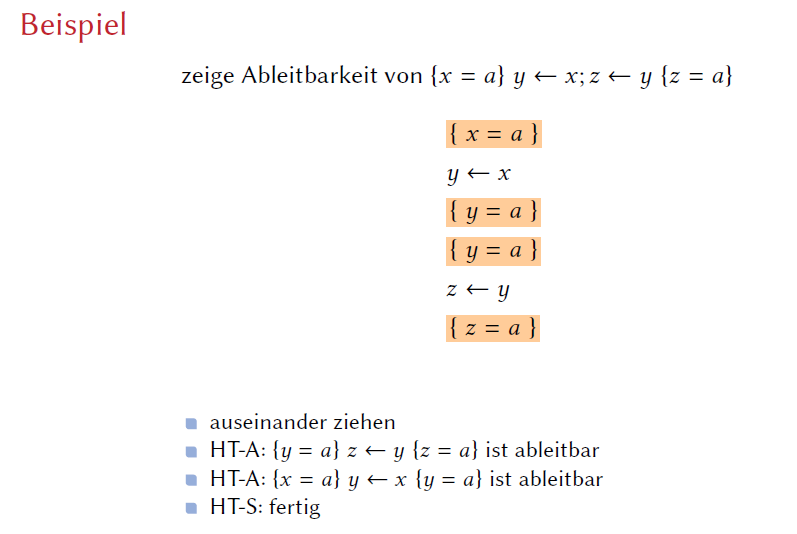
\includegraphics[scale=0.5]{hoare/bsp1}
\end{frame}

\begin{frame}{HT-I}
	\begin{minipage}{0.4\linewidth}
		\begin{align*}
			&\assert{ P } \\
			& \textbf{if } B \textbf{ then} \\
			&\hspace{2em} \assert{ P \wedge B } \\
			&\hspace{2em} S_1 \\
			&\hspace{2em} \assert{ Q }\\
			&\textbf{else} \\
			&\hspace{2em} \assert{ P \wedge \neg B } \\
			&\hspace{2em} S_2 \\
			&\hspace{2em} \assert{ Q }  \\
			&\textbf{fi}\\
			&\assert{Q }
		\end{align*}
	\end{minipage}
	\begin{minipage}{0.55\linewidth}
		\begin{block}{Regel HT-I \quad „If“}
			$\textbf{if } B\text{ } \textbf{ then } S_1 \textbf{ else } S_2 \textbf{ fi}$
			\smallskip
			\begin{itemize}
				\item Wenn $\{ P \wedge B \}\ S_1\ \{ Q \}$ gültig 
				\item und $\{ P \wedge \neg B \}\ S_2\ \{ Q \}$ gültig
				\item dann auch \\ $\{ P \} \textbf{ if } B \textbf{ then } S_1 \textbf{ else } S_2 \textbf{ fi } \{ Q \} $ gültig
			\end{itemize}
		\end{block}
%		\emph{HT4 : } $\textbf{if } B\text{ } \textbf{then } S_1 \textbf{ else } S_2 \textbf{ fi}$
%		\begin{itemize}
%			\item Wenn $\{ P \wedge B \} S_1 \{ Q \}$ gültig 
%			\item Wenn $\{ P \wedge \neg B \} S_2 \{ Q \}$ gültig
%			\item dann auch $\{ P \} \textbf{ if } B \textbf{ then } S_1 \textbf{ else } S_2 \textbf{ fi} \{ Q \} $ gültig
%		\end{itemize}
	\end{minipage}
\end{frame}

\begin{frame}{Beispiel: Berechnung von $\vert x \vert$}
	
	
	\begin{minipage}{0.4\linewidth}
		Erinnerung:
		\vspace{-.6\baselineskip}
		\begin{align*}
		&\assert{ P } \\
		& \textbf{if } B \textbf{ then} \\
		&\hspace{2em} \assert{ P \wedge B } \\
		&\hspace{2em} S_1 \\
		&\hspace{2em} \assert{ Q }\\
		&\textbf{else} \\
		&\hspace{2em} \assert{ P \wedge \neg B } \\
		&\hspace{2em} S_2 \\
		&\hspace{2em} \assert{ Q }  \\
		&\textbf{fi}\\
		&\assert{Q }
		\end{align*}
	\end{minipage}
	\begin{minipage}{0.4\linewidth}
		\begin{align*}
		&\assert{ x \in\R} \\
		&\textbf{if } x < 0 \textbf{ then } \\
		&\hspace{2em} \assert{ \visible<6->{ x\in\R\wedge x < 0 } } \\
		&\hspace{2em} \assert{ \visible<5->{ {-x} = \vert x \vert } } \\
		&\hspace{2em}  z \gets -x   \\
		&\hspace{2em} \assert{ \visible<2->{ z = \vert x \vert } } \\
		&\textbf{else} \\
		&\hspace{2em} \assert{ \visible<4->{ x\in\R\wedge x\geq 0 } } \\
		&\hspace{2em} \assert{ \visible<3->{ x = \vert x \vert } } \\
		&\hspace{2em} z \gets x \\
		&\hspace{2em} \assert{ \visible<2->{ z = \vert x \vert } } \\
		&\textbf{fi} \\
		&\assert{ z = \vert x \vert } 
		\end{align*}
	\end{minipage}
\end{frame}

\begin{frame}{Aufgabe}
	\vspace{-10mm}
	\begin{align*}
	&\assert{x=a \land y=b}  \\
	&\kw{if } x>y \kw{ then } \\
	&\hspace{2em} \assert{ \dots\ } \\
	&\hspace{2em}  z \gets y  \\
	&\hspace{2em} \assert{ \dots\ } \\
	&\kw{else } \\
	&\hspace{2em} \assert{ \dots\ } \\
	&\hspace{2em}  z \gets x  \\
	&\hspace{2em} \assert{ \dots\ } \\
	&\kw{fi } \\
	&\assert{z=\min(a,b)}
	\end{align*}
\end{frame}

\begin{frame}{Lösung}	
	\vspace{-2.5\baselineskip}
	\begin{alignat*}{2}
	&\assert{x=a \land y=b}  \\
	&\kw{if } x>y \kw{ then } \\
	&\hspace{2em} \assert{x=a \land y=b \land x>y} \\
	&\hspace{2em} \assert{y=\min(a,b)} \\
	&\hspace{2em}  z \gets y  \\
	&\hspace{2em} \assert{z=\min(a,b)} \\
	&\kw{else } \\
	&\hspace{2em} \assert{x=a \land y=b \land  \lnot (x>y)} \\
	&\hspace{2em} \assert{x=\min(a,b)} \\
	&\hspace{2em}  z \gets x  \\
	&\hspace{2em} \assert{z=\min(a,b)} \\
	&\kw{fi } \\
	&\assert{z=\min(a,b)}
	\end{alignat*}
\end{frame}


\mycomment{
%TODO: Lösung!!!
\begin{frame}{Jetzt seid ihr dran}
	\begin{align*}
	& z \gets x + y \\
	& z \gets z / 2 \\
	&\textbf{if } x \mod 2 = 0 \textbf{ then } \\
	&\hspace{2em} y \gets x + x \\
	&\hspace{2em} y \gets y / 4 \\
	&\textbf{else} \\
	&\hspace{2em} y \gets x - 1 \\
	&\hspace{2em} y \gets y / 2 \\
	&\textbf{fi} \\
	& z \gets z \· y \\
	&\assert{ z = div_2(a) \· (a+b)/2 } % WTF is div_2 ? => (2 `div`) ? a, b vs. x, y?
	\end{align*}
\end{frame}	
}


%\begin{frame}
%	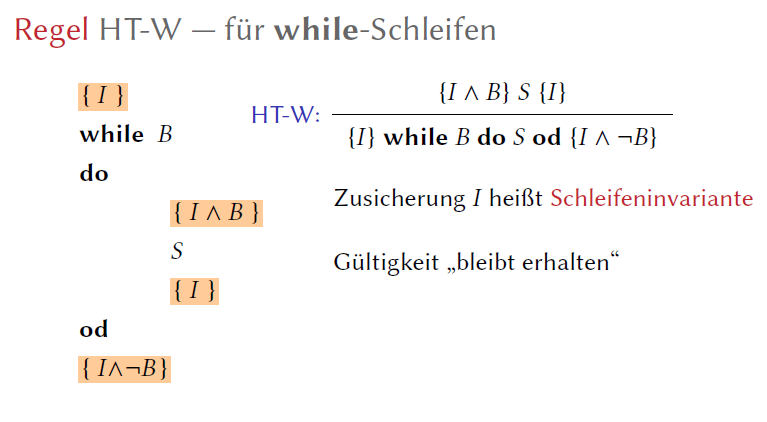
\includegraphics[scale=0.5]{hoare/htw}
%\end{frame}

\subsection{HT-W, Schleifeninvarianten}
\begin{frame}{HT-W}
	\begin{columns}[T] 
		\begin{column}[T]{.4\textwidth} 
			\vspace{-2\baselineskip}
			\begin{align*}
			&\assert{I} \q3uad \text{„Schleifeninvariante“} \\
			&\kw{while } B \kw{ do } \\
			&\qquad \assert{I \land B} \\
			&\qquad S \\
			&\qquad \assert{I} \\
			&\kw{od} \\
			&\assert{I \land \lnot B}
			\end{align*}
			\vspace{-1\baselineskip}
		\end{column}
		\begin{column}[T]{.4\textwidth} 
			\begin{block}{Regel HT-W \quad „While“}
				Wenn \htr{$I \land B$}{$S$}{$I$} gültig ist, dann ist auch die ganze \kw{while}-Schleife (s. links) gültig
			\end{block}
		\end{column}
	\end{columns}
	
	\pause
	\begin{block}{Schleifeninvarianten}
		\begin{itemize}
			\item sind Aussagen, die zu Beginn und Ende jedes Schleifendurchganges gültig sind
			\item helfen, die Korrektheit eines Programmes zu beweisen
			\item muss man ebenfalls beweisen 
			\item garantieren nicht die Korrektheit des Programms:\pause \\
			Terminierung der Schleife muss zusätzlich gezeigt werden! (nicht in GBI)
		\end{itemize}
	\end{block}
\end{frame}
	
\begin{frame}{Beispiel Schleifeninvarianten}
	\begin{columns}
	\begin{column}[T]{0.49\linewidth}
	\begin{align*}
		&\assert{x=a \land y=b}  \\
		&\assert{ \dots\ } \\
		&\kw{while } y\not=0 \kw{ do } \\
		&\qquad\assert{ \dots } \\
		&\qquad y \gets y-1 \\
		&\qquad\assert{ \dots } \\
		&\qquad x \gets x+1 \\
		&\qquad\assert{ \dots\ } \\
		&\kw{od } \\
		&\assert{ \dots\ } \\ \pause
		&\assert{x=a+b} \\
	\end{align*}
	\end{column} 
	
	\begin{column}[T]{0.5\linewidth}
		\visible<2->{
			\bigskip
			\begin{block}{Wertetabelle für $a=3$ und $b=4$}
				\centering
				\medskip
				\begin{tabular}{c|cc}	 
					Durchlauf $i$ & $x$ & $y$ \\ 
					\hline 
					0 & 3 & 4 \\
					1 & 4 & 3 \\
					2 & 5 & 2 \\
					3 & 6 & 1 \\
					4 & 7 & 0 \\
				\end{tabular}
			\end{block}
			\pause
			Schleifeninvariante: $$ x + y = a + b $$ 
		}
	\end{column}
	\end{columns}
\end{frame}

\begin{frame}{Beispiel Schleifeninvarianten – Lösung}
	\begin{minipage}{.4\linewidth}
		Erinnerung HT-W:
		\vspace{-.4\baselineskip}
		\begin{align*}
		&\assert{I}  \\
		&\kw{while } B \kw{ do } \\
		&\qquad \assert{I \land B} \\
		&\qquad S \\
		&\qquad \assert{I} \\
		&\kw{od} \\
		&\assert{I \land \lnot B}
		\end{align*}
	\end{minipage}
	\begin{minipage}{.4\linewidth}
		\begin{align*}
		&\assert{x=a \land y=b }  \\
		&\assert{ x+y=a+b }  \\
		&\kw{while } y\not=0 \kw{ do } \\
		&\qquad\assert{x+y=a+b \land y\not=0 }  \\
		&\qquad\assert{x+1+y-1=a+b } \\
		&\qquad y \gets y-1 \\
		&\qquad\assert{x+1+y = a+b} \\
		&\qquad x \gets x+1 \\
		&\qquad\assert{ x+y = a+b} \\
		&\kw{od } \\
		&\assert{ x+y = a+b \land y=0 } \\
		&\assert{x=a+b} \\
		\end{align*}
	\end{minipage}
	
\end{frame}

\begin{frame}{Exkurs: Schl.-Inv. mit Vollst. Induktion}
	Wir zeigen mit vollständiger Induktion die Gültigkeit der Schleifeninvariante. Dabei sei $i$ die Anzahl der bisher durchgelaufenen Schleifendurchläufe.\\
	
	\emph{Behauptung}: $$ \forall\ i \in \{0,...,b\} : x_i + y_i = a+b $$ \pause
	\begin{block}{Induktionsanfang}
		Für $i=0$ gilt $ x_0+y_0 = a+b $ nach Vorbedingung.
	\end{block} \pause 
	\begin{block}{Induktionsvorrausetzung}
		Für ein beliebig aber festes $i\in \{0,...,b\}$ gelte die Behauptung.
	\end{block}
\end{frame}

\begin{frame}{Exkurs: Schl.-Inv. mit Vollst. Induktion}
	\vspace{-2\baselineskip}
	\begin{align*}
	&\assert{x=a \land y=b}  \\
	&\assert{ x+y=a+b }\\
	&\kw{while } y\not=0 \kw{ do } \\
	&\qquad y \gets y-1 \\
	&\qquad x \gets x+1 \\
	&\kw{od } \\
	&\assert{x=a+b} \\
	\end{align*}
	\vspace{-2\baselineskip}
	\begin{block}{Induktionsschluss}
		Zu zeigen: $ x_{i+1} + y_{i+1} = a+b $ \pause
	%\vspace{-1.3\baselineskip}
		\begin{align*}
		x_{i+1}+y_{i+1} &= x_i +1 + y_i -1 \\
		&= x_i + y_i \\
		&\overset{IV}{=} a+b.
		\end{align*}
	\end{block}
\end{frame}

\begin{frame} {Weitere Beispiele}
	Weitere Beispiele findet ihr hier: Übung 8, WS 15/16
\end{frame}


% next time \section{Endliche Akzeptoren}
\begin{frame}[t]{Endliche Akzeptoren}
	\begin{Definition}
		Ein \textbf{endlicher Akzeptor} $A$ ist ein \emph{Moore}-Automat mit Ausgabealphabet $ Y= \{\word 0,\word 1\}$, der zuletzt $\word 1$ ausgibt, falls ihm das Wort gefällt und \word 0 sonst.
	\end{Definition} 
	
	$A$ \textbf{akzeptiert} ein Wort $w$, wenn er als Letztes eine $\word 1$ ausgibt. \\ \medskip 
	
	\only<all:2>{
		\begin{center}
					\begin{tikzpicture}[->,>=stealth,shorten >=1pt,auto,node distance=1.8cm,
				semithick,initial text={}]
				\tikzstyle{every state}=[]
				
				\node[state] (A)                    {$a\io\word 0$};
				\node[state] (B) [right of=A] 	    {$b\io\word 1$};
				
				\end{tikzpicture}
		\end{center}
	}
	\only<all:3>{
		\begin{center}
					\begin{tikzpicture}[->,>=stealth,shorten >=1pt,auto,node distance=1.8cm,
				semithick,initial text={}]
				\tikzstyle{every state}=[]
				
				\node[state] (A)                    {$a$};
				\node[state, accepting] (B) [right of=A] {$b$};
				
				\end{tikzpicture}
		\end{center} 
		\emph{Notation:} Wir nennen die Menge der \textbf{akzeptierenden Zustände} $F$ und malen solche mit einem Doppelkreis. \\ 
	}
\end{frame}

\begin{frame}{Von einem Akzeptor erkannte Sprache}
	Wir sprechen von einer \textbf{akzeptierten Sprache} über einem Alphabet. Sie ist definiert als 
	\begin{align*}
		L(A) &:= \{ w \mid f_*(z_0,w) \in F \}  \\
			 &\: = \{ w \mid g_*(z_0,w) = \word 1 \}.
	\end{align*}
	Also sind in einer akzeptierten Sprache alle Wörter, die von $A$ akzeptiert werden. \pause
	
	\begin{Beispiel}
		Sei $A$ gegeben als
		\vspace{-2\baselineskip}
		\begin{center}
			\begin{tikzpicture}[->,>=stealth,shorten >=1pt,auto,node distance=1.8cm,
			semithick,initial text={}]
			\tikzstyle{every state}=[]
			
			\node[initial, state, accepting] (A)                    {$z_0$};
			\node[state] (B) [right of=A] {$z_1$};
			
			\path
				(A) edge [loop above] node {\word a, \word b}  (A)
					edge [bend right=7] node [below] {\word c} 		  (B)
				(B) edge [loop right] node {\word c}		  (B)
					edge [bend right=7] node [above] {\word a, \word b} (A)
			;
			\end{tikzpicture}. % Sätze enden mit nem Punkt! :D
		\end{center} 
		\pause
		Dann ist $L(A) = \set{w \in \set{\word a, \word b, \word c}^* \Mid \text{$w$ endet nicht auf \word c}}$.
	\end{Beispiel}
\end{frame}

\begin{frame}{Aufgaben}
	Gebt einen Akzeptor an, der die Sprache aller Binärzahlen erkennt, die Zweierpotenzen darstellen. 
	\pause ($= \set{\word 0}^* \* \set{\word 1} \* \set{\word 0}^*$) \\
	%\vspace{-2\baselineskip}
	\begin{center}
		\begin{tikzpicture}[->,>=stealth,shorten >=1pt,auto,node distance=2cm,
		semithick,initial text={}]
		\tikzstyle{every state}=[]
		
		\node[initial,state] (A)                    {$a$};
		\node[state,accepting] (B)  [right of=A]     {$b$};
		\node[state]		 (M)  [right of=B]		{$m$};
		
		\path
		(A) edge [loop above]  node {\word 0} (A) 
		(A) edge 			  node {\word 1} (B) 
		(B) edge [loop above]  node {\word 0} (B) 
		(B) edge 			  node {\word 1} (M) 
		(M) edge [loop above] node {\word 0, \word 1} (M);
		\end{tikzpicture}
	\end{center}
	\pause
	\begin{block}{Bonusaufgabe}
		Gebt einen Akzeptor an, der die Sprache aller geraden Binärzahlen erkennt. 
		\pause ($= \set{\word 0,\word 1}^* \* \set{\word 0}$) \\
		%\vspace{-2\baselineskip}
		\begin{center}
			\begin{tikzpicture}[->,>=stealth,shorten >=1pt,auto,node distance=1.8cm,
			semithick,initial text={}]
			\tikzstyle{every state}=[]
			
			\node[initial, state] (A)                    {$a$};
			\node[state, accepting] (B) [right of=A] {$b$};
			
			\path
			(B) edge [loop above] node  {\word 0}  (B)
				edge [bend right=7] node [above] {\word 1} 		  (A)
			(A) edge [loop above] node  {\word 1}		  (A)
				edge [bend right=7] node [below] {\word 0} (B)
			;
			\end{tikzpicture}
		\end{center} 
	\end{block}
\end{frame}

\begin{frame}{Aufgabe}
	Der endliche Akzeptor $A = (Z, z_0, X, f, F)$ sei gegeben durch
	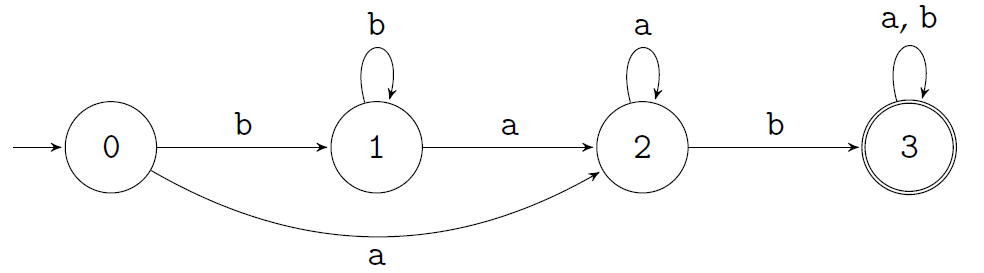
\includegraphics[scale=0.4]{automaten/akz1516B12A1}
	
	Gebt die von $A$ akzeptierte Sprache $L(A)$ unter ausschließlicher Benutzung der formalen Sprachen $\{\word a\}$, $\{\word b\}$, sowie $\{\word a, \word b\}$, des Konkatenationsabschlusses und des Produkts formaler Sprachen an.
	
	\emph{Beispiel:} $\{\word a, \word b\}^* \cdot \{\word a\} \cdot \{\word b\}$
	
	\visible<2-|handout:2>{
		\begin{block}{Lösung}
			$L(A) = \{\word b\}^* \cdot \{\word a\} \cdot \{\word a\}^* \cdot \{\word b\} \cdot \{\word a, \word b\}^*$ \\
			$\hphantom{L(A) } = \{\word b\}^* \cdot \hphantom{\{\word a\} \cdot \mbox{}} \{\word a\}^+ \!\cdot \{\word b\} \cdot \{\word a, \word b\}^*$
		\end{block}
	}
\end{frame}

\begin{frame}{Bonusaufgabe}
	\begin{enumerate}[a)]
		\item Zeichnet einen möglichst kleinen endlichen Akzeptor mit $ X = \{\word a, \word b\}$, der alle Wörter akzeptiert, bei denen die Anzahl der $\word a$ durch $5$ teilbar ist.
		\item Zeichnet einen Akzeptor mit $ X = \{\word a,\word b\}$, der alle Wörter akzeptiert, in denen nirgends hintereinander zwei $\word b$ vorkommen.
	\end{enumerate}		
\end{frame}

\begin{frame} {Lösung Bonusaufgabe a)}
	\begin{figure}[H] 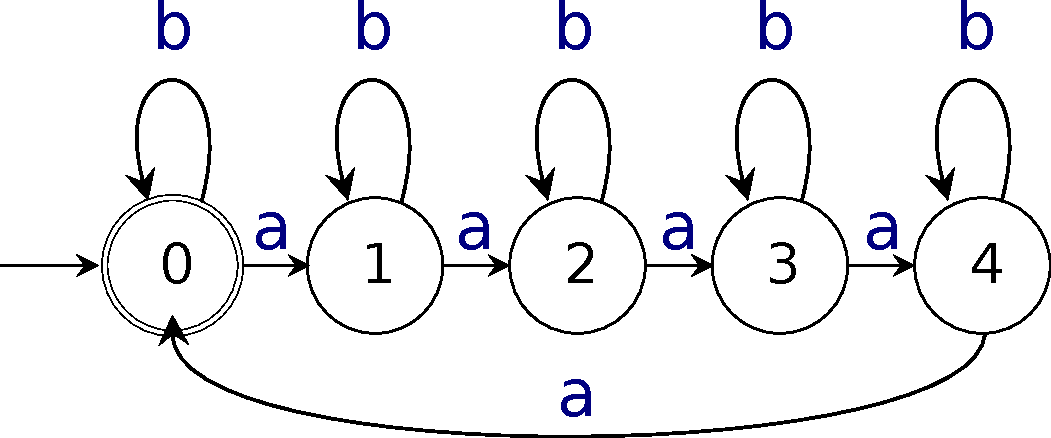
\includegraphics[scale=0.5]{automaten/Akzeptor1.pdf} \end{figure}		
\end{frame} 

\begin{frame}{Lösung Bonusaufgabe b)}
	\begin{figure}[H] 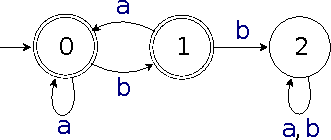
\includegraphics[scale=1.5]{automaten/Akzeptor2.pdf} \end{figure}
\end{frame}



% ---------

\mycomment{
% WiSe 10/11 Aufgabe 6 c 
\begin{frame}{Übung: Akzeptoren}
	Die Sprache $L\subseteq \{\word a,\word b\}^\ast $ sei definiert als die Menge aller Wörter $w$, die folgende Bedingungen erfüllen:
	\begin{align*}
	N_{\word b}(w) &> N_{\word a}(w)\\ 
	\forall v_1,v_2 \in \{\word a,\word b\}^\ast : \qquad w &\neq v_1 \word{bb} v_2 
	\end{align*}
	
	Gebt einen endlichen Akzeptor an, der $L$ erkennt. \\
	
	\bigskip
	\pause
	\begin{block}{Tipps}
		\begin{itemize}[<+->]
			\item Die zweite Bedingung bedeutet: Das Wort darf nirgends zwei \word b hintereinander enthalten.
			\item Was passiert, wenn das Wort mit einem \word a beginnt?\\
			Kann das Wort noch akzeptiert werden?
		\end{itemize}
	\end{block}
\end{frame}

\begin{frame}{Übung: Akzeptoren: Lösung}
	\begin{figure}
		\centering
		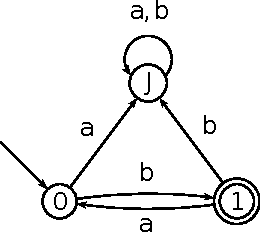
\includegraphics[width=0.7\linewidth]{automaten/Loesung2.pdf}
	\end{figure}
\end{frame}
}

\begin{frame}	
	\begin{block}{Was ihr nun wissen solltet}
		\begin{itemize}
			\item Wie man die Laufzeit von TMs beurteilt
			\item Was \textbf{P} und \textbf{PSPACE} sind
		\end{itemize}
	\end{block}
	
	\begin{block}{Was nächstes Mal kommt}
		\begin{itemize}
			\item Wie man die Korrektheit von Algorithmen beweist
			\item Wie man die Effizienz von Algorithmen beurteilt
			\item Endlich: Graphen
			%\item Ein Regelwerk für einen Ausdruck -- Reguläre Ausdrücke
			%\item Rechtslineare Grammatiken
			%\item Turingmaschinen -- mächtiger wird es nicht mehr!
		\end{itemize}
	\end{block}
\end{frame}


\xkcdframe{287}{Danke für eure Aufmerksamkeit! \smiley}{2.5}
%\lastframe{0.6}{30}{xkcd/automation_1319.png}{http://www.xkcd.com/1319}
%\xkcdframe{0.5}{30}{xkcd/houston_1438.png}{http://www.xkcd.com/1438}{Oh, hi mom. No, nothing important, just work.}



\slideThanks

\end{document}